\chapter{Computational Methods} \label{ch:3}

In this chapter, I will explain some relevant background between two of the computational techniques I've used in this work: the particle-in-cell method and machine learning.

\section{The Particle-In-Cell Method}

The \gls{PIC} method involves solving Maxwell's Equations on a grid 

\begin{align}
	\nabla \cdot \vec{E} &= \frac{\rho}{\epsilon_0}  \label{eq:gauss} \\
	\nabla \times \vec{E} &= - \frac{\partial \vec{B}}{\partial t} \label{eq:faraday} \\
	\nabla \cdot \vec{B} &= 0 \label{eq:gauss_magnetism} \\
	\nabla \times \vec{B} &= \mu_0 (\vec{J} + \epsilon_0 \frac{\partial \vec{E}}{\partial t}) \label{eq:ampere}
\end{align}
This is combined with the lorentz force

\begin{equation}
	\vec{F} = q(\vec{E} + \vec{v} \times \vec{B}) \label{eq:lorentz_pic}
\end{equation}
which determines the motions (i.e. $\vec{r}$ and $\vec{v}$) of charged particles by integration. It is impossible to keep track of every single particle in this type of simulation (roughly on the order of Avogadro's number $\sim 10^{23}$). Instead, we lump many particles together into what is called a \emph{macro particle}. For example, one macro electron could represent 1 trillion real electrons. Spatially, we must separate the simulation volume into a grid where each cell has length $\Delta x$, $\Delta y$, and $\Delta z$ in the x, y, and z direction respectively. Temporally, we introduce a time step $\Delta t$ which allows us to propagate Maxwell's Equations forward in time by $\Delta t$ for every iteration.

For simplicity, non-relativistic equations will be introduced in this section, but they can easily be generalized to the relativistic versions which are implemented in modern PIC codes. Additionally, some of the equations will assume a 2D grid, but a 3D grid is similarly straightforward to generalize.

\subsection{Densities and Shape Factors}

At each time step in a simulation, the particles will have a defined position and velocity. The charge density $\rho_{i,j}$ (for the cell at the $i^\text{th}$ and $j^\text{th}$ grid point in the x and y directions) can be computed as the sum of all the charges $q_\alpha$ contained in the cell at grid point $(i,j)$ divided by the cell area: $\rho_{i,j} \equiv \frac{\sum_\alpha q_\alpha}{\Delta x \Delta y}$\footnote{This is for a 2D geometry where we implicitly divide by 1 m to get the units right. In 3D, the denomenator would have $\Delta z$ as well}. The current density $\vec{J}_{i,j}$ can be obtained similarly -- $\vec{J}_{i,j} \equiv \frac{\sum_\alpha q_\alpha \vec{v}_\alpha}{\Delta x \Delta y}$. Assigning the densities to the nearest grid point in this manner is sensibly called \gls{NGP} by Birdsall and Langdon \cite{Birdsall_2004_PIC}.

Since the PIC approach contains many real particles for each macro particle, it is desired to smooth the macro particle densities throughout adjacent cells. We can modify the individual density contributions of particles by a shape factor $S(\vec{r_\alpha} - \vec{r})$ that depends on a particle's location $\vec{r_\alpha}$ in relation to a grid point located at $\vec{r}$. This shape factor is normalized so that integrating over the area of the simulation yields 1 to ensure the particle number is properly being conserved. The simplest improvement over \gls{NGP} would be the \emph{top hat} shape factor (also called Cloud in Cell \cite{Birdsall_2004_PIC}) which assigns density contributions proportional to proximity of the nearest cells within ($\Delta x$,$\Delta y$). This has the shape of a uniform distribution and thus looks like a ``top hat'' in 1D. It is a $0^\text{th}$ order shape factor and can be represented by the following equation

\begin{equation}
	S_0(x) \equiv \begin{cases}
		1 & \text{if } \lvert x \rvert \leq 0.5 \Delta x \\
		0 & \text{otherwise}
	\end{cases} \label{eq:tophat}
\end{equation}
A further improvement will weight the particles closer to a particular grid point higher than a particle further away. If this weighting is linear over an area ($2 \Delta x$, $2 \Delta y$), it is called the \emph{triangle} shape factor and reprsented by the following equation in 1D

\begin{equation}
	S_1(x) \equiv \begin{cases}
		1-\frac{\lvert x \rvert}{\Delta x} & \text{if } \lvert x \rvert \leq \Delta x \\
		0 & \text{otherwise}
	\end{cases} \label{eq:triangle}
\end{equation}
It turns out that the higher order shape factors $S_n(x)$ can be represented by convolutions of $S_0(x)$ 

\begin{figure}
	\centering 
	\includegraphics[width=0.6\linewidth]{planning/images/shape_functions.png}
	\caption{The top hat ($S_0(x)$), triangle ($S_1(x)$) and $3^\text{rd}$ order spline ($S_3(x)$) are plotted in 1D.}
	\label{fig:shape_factors}
\end{figure}

\begin{equation}
	S_n(x) \equiv \int_{-\infty}^\infty S_{n-1}(x')S_0(x-x') dx'
\end{equation}
and the shape factors for $n \geq 2$ are commonly called n-splines. The third order spline is used in this work and weights particles over an area ($4 \Delta x$, $4 \Delta y$) and is represented in 1D by 

\begin{equation}
	b_3(x) = \begin{cases}
		\frac{1}{6}(8 - 12 \lvert \tilde{x} \rvert + 6 \tilde{x}^2 - \tilde{x}^3) & \text{if } 1 \leq \lvert \tilde{x} \rvert \leq 2 \\
		\frac{1}{6}(4 - 6 \tilde{x}^2 + 3 \tilde{x}^3) & \text{if } \lvert \tilde{x} \rvert \leq 1 \\
		0 & \text{otherwise}
	\end{cases}
\end{equation}
where $\tilde{x} \equiv x / \Delta x$ normalizes the position $x$. See \autoref{fig:shape_factors} for a comparison of the three shape factors. These shape factors not only apply to the calculation of densities, but also to the electric and magnetic fields. In this way, the fields used to update particle positions and velocities are averaged over neighboring cells. Although higher-order shape factors can increase computational demands, smoother charge and current densities result in more accurate fields and reduce the number of macroparticles required. As shown in \autoref{sec:app1}, field calculation errors will compound over time to worsen energy conservation which can be mitigated by adopting a higher-order shape factor\footnote{In their paper that describes the EPOCH PIC code, Arber et. al. \cite{Arber_2015_PPCF} says ``top-hat shape functions should never be used for laser-solid simulations''}. 

\subsection{Field Solver and Particle Push}

\begin{figure}
	\centering 
	\includegraphics[width=0.8\linewidth]{planning/images/yee_grid.PNG}
	\caption{The ``Yee'' grid is depicted (left) where the electric and magnetic field components are staggered by half a cell. The fields, currents, position, and velocity make use of the staggered grid by leapfrog time integration (right). This picture was taken from the WarpX documentation \cite{WarpX_documentation} (which is another PIC code).}
	\label{fig:yee_grid}
\end{figure}

The \gls{PIC} method is able to make efficient use of the second order accurate central difference approximation to compute derivatives. A simpler method like Euler integration is only first order accurate and will suffer in terms of accuracy. Higher order methods like 4th order Runge-Kutta have much higher computational costs in terms of operations per time step and memory consumption. The central difference scheme is accomplished by alternately calculating electric and magnetic fields, staggered by half a time step, in an approach called \emph{leapfrog integration} \cite{Birdsall_2004_PIC}. This can be seen in the right half of \autoref{fig:yee_grid} where the calculations of $E$ and $J,B$ alternate in a ``leapfrog'' fashion. It turns out that this staggering also comes with some nice properties like automatically satisfying \autoref{eq:gauss_magnetism}. By rearranging \autoref{eq:faraday}, we can update the electric and magnetic fields through the following equations \cite{Arber_2015_PPCF}

\begin{align}
	\vec{E}^{n+1} &= \vec{E}^{n} + \Delta t (c^2 \nabla \times \vec{B}^{n+\frac{1}{2}} - \frac{1}{\epsilon_0} \vec{J}^{n+\frac{1}{2}}) \label{eq:E_update} \\
	\vec{B}^{n+\frac{1}{2}} &= \vec{B}^{n-\frac{1}{2}} - \Delta t (\nabla \times \vec{E}^{n}) \label{eq:B_update}
\end{align}
where $\vec{J}^{n+\frac{1}{2}} \equiv \frac{\sum_\alpha q_\alpha \vec{v}^{n+\frac{1}{2}}_\alpha}{\Delta x \Delta y}$ depends on the velocity. The updated velocity for each particle is calculated through the force from \autoref{eq:lorentz_pic}. 

\begin{equation}
	\frac{v^{n + \frac{1}{2}}_\alpha - v^{n - \frac{1}{2}}_\alpha}{\Delta t} = \frac{q}{m}[E^n_\alpha + \frac{v^{n + \frac{1}{2}}_\alpha + v^{n + \frac{1}{2}}_\alpha}{2} \times B^n_\alpha] \label{eq:v_update}
\end{equation}
The $\alpha$ subscript indicates the quantities are calculated for each particle; thus, the fields are smoothed out by the shape factor (e.g. $E^n_\alpha \equiv \int E^n S_3(x-x_\alpha, y-y_\alpha, z-z_\alpha) \; dx \; dy \; dz$). In practice, Equations \eqref{eq:B_update} and \eqref{eq:E_update} are broken up into half-steps so that the electric and magnetic field are known for all half-steps. At first glance, \autoref{eq:v_update} does not appear to have an explicit solution for $v^{n + \frac{1}{2}}$. There are implicit methods that can solve this equation like \gls{LSP} \cite{Welch_2004_LSP}. It turns out that there is an explicit solution given by the \emph{Boris Rotation Algorithm}. If we define 

\begin{align}
	v^{n + \frac{1}{2}} &= v^+ + \frac{q E^n}{2 m} \Delta t \label{eq:vplus} \\
	v^{n - \frac{1}{2}} &= v^- - \frac{q E^n}{2 m} \Delta t \label{eq:vminus}
\end{align}
we can separate out the electric field dependence to get 

\begin{equation}
	\frac{v^+ - v^-}{\Delta t} = \frac{q}{m}[\frac{v^+ + v^-}{2} \times B]
\end{equation}
which can conveniently be calculated through a rotation \cite{Birdsall_2004_PIC} through the following steps:

\begin{enumerate}
	\item Compute $v^-$ from \autoref{eq:vminus}.
	\item Compute $\vec{t} \equiv \frac{q \Delta t}{2 m} \vec{B}^n $ (equivalent in magnitude to $\tan(\theta/2)$ where $\theta$ is the rotation angle)
	\item Compute $\vec{s} = \frac{2 \vec{t}}{1 + t^2}$ (equivalent in magnitude to $\sin(\theta/2)$)
	\item Compute $\vec{v}' = \vec{v}^- + \vec{v}^- \times \vec{t}$.
	\item Compute $\vec{v}^{n+\frac{1}{2}}$ from \autoref{eq:vplus}.
\end{enumerate}
Now, the particles can be advanced or ``pushed'' from

\begin{equation}
	x^{n+1} = x^{n} + v^{n+\frac{1}{2}} \Delta t \label{eq:particlepush}
\end{equation}
Note that the position and velocity are staggered by a half step in the same leapfrog integration scheme as the fields as illustrated in \autoref{fig:yee_grid}. For completeness, the velocity initially needs to be pushed backwards from $v^{0} \rightarrow v^{-\frac{1}{2}}$. This is not done in a time-centered way, but is only needed at the start of the simulation. 

\section{Machine Learning}
What is \gls{ML}? According to the computer scientist Arthur Samuel who popularized the term in 1959 \cite{Geron_2023_ML}, it is the 

\begin{quote}
	... field of study that gives computers the ability to learn without being explicitly programmed. 
\end{quote}
The book \emph{Hands-On Machine Learning with Scikit-Learn} by Aurelien Geron \cite{Geron_2023_ML} gives a simple example of how a \gls{ML} model differs from a more traditional computer program in the form of an email spam filter. A traditional filter would implement user specified rules that mark emails as spam based on e-mail address and subject line keywords for example. A \gls{ML} approach would determine what keywords and e-mail addresses to look for based on prior emails that have been flagged as spam.

The key difference in the two approaches is predictive power. The traditional filter removes spam from messages that fit a pattern explicitly given by the user. The \gls{ML} filter learns a generalized model that predicts possibly unforeseen types of spam. Since the \gls{ML} model has more degrees of freedom, it is more susceptible to incorrect predictions. In this section, we'll overview how to handle data for \gls{ML} algorithms, compare model training for different methods, and explain how these models can be used in practice. The information below is largely from the book by Geron \cite{Geron_2023_ML} unless specified otherwise.

\subsection{Pre-processing}
\gls{ML} can be either supervised or unsupervised based on whether the data is labeled with a particular output. In the \gls{ML} context, model outputs are often referred to as labels and model inputs are often referred to as features. For the e-mail classification example, a supervised model would have training data that is already labeled as spam (or not spam) and an unsupervised model would have to infer if the data is spam by other means (e.g. clustering similar emails together). We will not be considering unsupervised learning in this work because we are ultimately interested in labeled data (which would be electron or proton energy spectra). To train an \gls{ML} model effectively, there are various things that need to be taken into account: 

\begin{itemize}
	\item Data Quantity: We need a significant amount of data in order to learn relevant trends and patterns. For example, a good spam classifier would have many e-mails (thousands to millions) to train on.
	\item Representative Data: The data should be representative of all data points. A spam classifier trained only on data prior to 2010 will not accurately predict modern spam emails.
	\item Poor-Quality: The data should not have significant errors, outliers, and noise. 
	\item Irrelevant Features: The input data (features) to the model should all be relevant. For example, taking into account the exact time that a spam e-mail is received may not be the most relevant as spam emails are often sent out at random times. 
\end{itemize}
Failure to take the preceding steps into account can oftentimes lead to one of two things

\begin{itemize}
	\item Overfitting: This can happen when the data is too complex in relation to the data. An example would be using a polynomial to fit a set of points that fall on a straight line. To fix this, we can constrain the model to make it more simple, gather more training data, or reduce noise in the training set.
	\item Underfitting: This is when the model is too simple in relation to the data. This can be fixed by selecting a more complex model, using better features, and reducing any constraints on the model.
\end{itemize} 
Machine learning models are often more effective if we can perform \emph{pre-processing} which is the set of actions that transform raw data into data ready to be fed into a \gls{ML} model. As will be discussed in \autoref{ch:6}, significant pre-processing was needed which included removing missing values, combining data sources, applying a median-based filter, compressing the spectra into two metrics, and more. One particularly effective method of pre-processing that is specific to \gls{ML} is data normalization which makes sure that all the features and labels are approximately on the same scale. The two most common ways to approach this are summarized below: 

\begin{itemize}
	\item Standard Scaling: A particular feature can be transformed through the following: $x_i \rightarrow \frac{x_i - \mu}{\sigma}$ where $\mu$ is the mean of all the data points $x_i$ and $\sigma$ is the standard deviation. This normalizes the data to be centered at 0 and have a standard deviation of 1. 
	\item Min Max Scaling: A particular feature can be transformed by setting the minimum value to 0, the maximum value to 1, and all values in between would be linearly proportional. 
\end{itemize}
The Min Max Scaling is useful when the data is known to be uniformly distributed with a fixed minimum and maximum. The Standard Scaling is more general and works best if the data is normally distributed. 

\subsection{Model Selection}
Given a pre-processed dataset, some additional steps are needed before deploying a \gls{ML} model. There are many different types of models one can select and even a particular model can have different so-called \emph{hyperparameters} that characterize it. For example, a hyperparameter of the polynomial regression model is the degree. A standard approach to model selection is through \emph{cross-validation} which breaks up a dataset into different partitions and varies which ones are used for training and which are used for model evaluation. If a model has good performance with one partition but not with another, then the model will not likely generalize well with additional data. In the \emph{cross-validation} process we only want to use data from a specified training set and not from a different testing set that we want to make useful predictions on. A typical training-testing split is 80-20\% (which is what was used in \autoref{ch:5}). 

To implement cross-validation, we pick a number of partition arrangements for the training set and evaluate the model performance for each partition for a number of hyperparameter combinations. For the polynomial regression example, we could evaluate the average error between 5 partition arrangements for polynomial degree ranging from 2 to 7 and pick the model that has the lowest amount of error. In python, we use the \texttt{GridSearchCV} module of scikit-learn \cite{Pedregosa_2011_Scikit-Learn} package to handle cross-validation for a ``grid'' of hyperparameter combinations for polynomial and other models as discussed in the next subsection.

To evaluate model performance, one needs to choose an error (or accuracy) metric. Two common error metrics are the \gls{MSE} and the \gls{MAPE} which are defined as follows: 

\begin{align}
	\text{MSE} &\equiv  \frac{1}{N} \sum_{i=1}^N (y_i - \hat{y}_i)^2 \\
	\text{MAPE} &\equiv \frac{1}{N} \sum_{i=1}^N \lvert \frac{y_i - \hat{y}_i}{y_i} \rvert
\end{align}
where $y_i$ is a particular output value, $\hat{y}_i$ is the \gls{ML} model prediction, and $N$ is the number of points in the dataset. By defining these error metrics, the model with the lowest cross-validation error should be the best model. 

\subsection{Model Types}

A polynomial is one simple model that involves minimizing the \gls{MSE} between data values and model predictions of the following formula: 

\begin{equation}
	\hat{y} = \beta_{0,0} + \beta_{1,0} x_1 + \beta_{0,1} x_2 + \beta_{1,1} x_1 x_2 + \cdots
\end{equation}
where $\beta_{i,j}$ are the polynomial coefficients. This equation incorporated two inputs $x_1$ and $x_2$ but can be generalized for any number of inputs. These coefficients can be found by a least-squares minimization algorithm \cite{Geron_2023_ML}. 

In principle, any dataset can be fit by a polynomial model of a sufficiently high degree. However, such a model would be prone to overfitting -- a good model with predictive power should be able to predict data not yet seen. Wolpert \cite{Wolpert_1997_IEEE} famously showed in his 1996 paper that if we don't make any assumptions about the data at hand, then there is no reason to prefer a particular \gls{ML} model over another. This is sometimes referred to as the \emph{no free lunch} theorem. Therefore, it is always instructive to experiment with a variety of models to see which one works best. 

Instead of a polynomial, more sophisticated regression models can be used like the ridge regression which uses a regularization hyperparameter to avoid overfitting. Similarly, \gls{SVR} (which falls in the class of support vector machines) uses a regularization parameter that tries to maximize the number of data points that are close to the prediction within some margin. A big advantage of the \gls{SVR} is that it can utilize the so-called ``kernel trick'' which allows the model to use higher dimensional features (like the polynomial model), but without explicitly calculating all the higher order components. Importantly, this has both time and memory saving implications. A common ``kernel'' is the \gls{RBF} which calculates a similarity measure between two data points involving a dot product and is easy to compute. 

Another regression method that can make use of the kernel trick is the Gaussian Process -- a method that doesn't just construct one function to fit the data, but rather a distribution of functions that all fit the data. The functions can effectively be averaged to create a \gls{GPR} or an uncertainty can be quantified by taking a standard deviation of the distributions at a particular point. These are particularly useful in the context of \gls{BO} where the uncertainty information can inform new parameters to explore when data is expensive or difficult to obtain.

\begin{figure}
	\centering 
	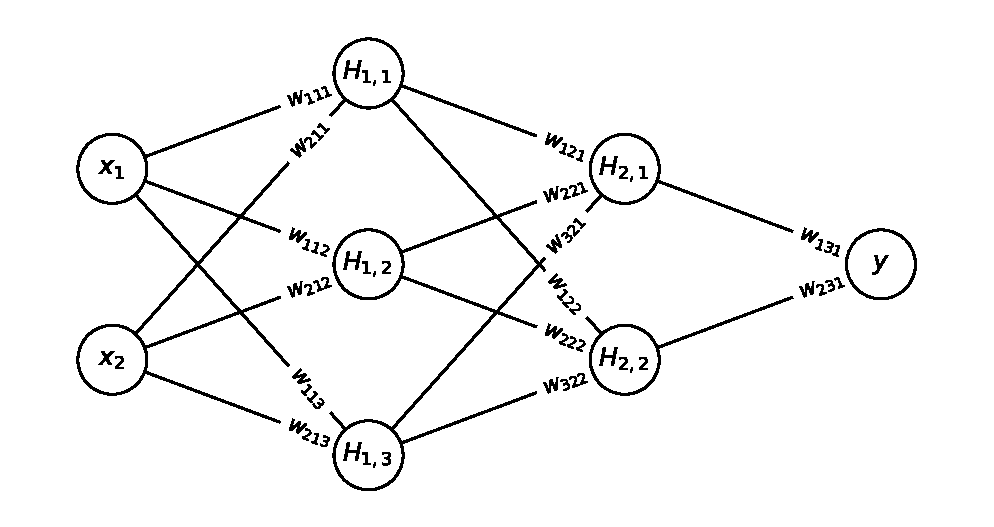
\includegraphics[width=0.8\linewidth]{planning/images/nn_basic.eps}
	\caption{A neural network architecture with labeled weights between the nodes in adjacent layers. This network has 2 inputs, 1 output, and 2 hidden layers (which have 3 or 2 nodes in each).}
	\label{fig:nn_basic}
\end{figure}

A more general purpose model capable of learning functions of high complexity is the \gls{NN}. This model, just like a linear regression, fits an intercept and coefficients to each input variable. However, the \gls{NN} chains many of these linear regressions together -- that is the output of one linear regression becomes the input of the next linear regression. The intermediary outputs are computed in the \emph{hidden layers}. Since a sequence of linear regressions will only produce another linear regression, \emph{activation functions} are needed to introduce non-linearity between the layers. The simplest activation function is the \gls{ReLU} which is defined as

\begin{equation}
	\text{ReLU}(x) =
	\begin{cases}
	 x &\text{ if } x > 0 \\
	 0 &\text{ otherwise }
	\end{cases}
\end{equation}  
To illustrate how this model works, one can look at \autoref{fig:nn_basic}. This network shows nodes that are connected by weights $w_{ijk}$ where $i$ is the vertical position of the node in the previous layer, and $j$ is the numbered hidden layer, and $k$ is the vertical position of the node in the current layer. To calculate $H_{1,1}$ for example, one would take a sum of the inputs multiplied by corresponding weights with an additional bias term (and then apply an activation function)

\begin{equation}
	H_{1,1} = \text{ReLU}(b_{11} + w_{111} x_1 + w_{211} x_2)
\end{equation}
or more generally $H_{1,k} = b_{1k} + \sum_{i} w_{i1k} x_i$. To calculate $H_{2,1}$ one would need to add up the contributions from $H_{1,1}$, $H_{1, 2}$, and $H_{1, 3}$

\begin{equation}
	H_{2,1} = \text{ReLU}(w_{121} H_{1,1} + w_{221} H_{1,2} +w_{321} H_{1,3})
\end{equation}
In this way, the intermediary hidden layers provide a number of free parameters equal to the number of weights $w_{ijk}$ (the number of edges) added to the number of bias terms $b_{ijk}$ (the total number of nodes excluding the input layer). Due to the interconnected nature of the model, the output will depend on every edge weight that is along the path from an input node to the specified output node. To train the \gls{NN}, one can employ the method of \emph{gradient descent}. This involves calculating the gradient of a designated error metric (like the \gls{MSE}) with respect to the model parameters (weights and biases). These gradients inform how the model should be updated to minimize the \gls{MSE}. If $\theta$ is a model parameter, this update is given as 

\begin{equation}
	\theta_\text{new} = \theta_\text{old} - \eta \nabla_\theta \text{MSE}(\theta) \label{eq:gradient_descent}
\end{equation}
Here, $\eta$ is called the \emph{learning rate} which is a scale factor that controls the magnitude of the update. This is an iterative procedure where at each step, the model output is calculated and the weight updates are computed from the gradients\footnote{The model output calculation is sometimes called the ``forward pass'' and gradient update is sometimes called the ``backward pass'' or ``back-propagation''.}. Each of these iterations is called an \emph{epoch} which can furthermore be divided by training the data in multiple batches (instead of all the data with one pass). The training process can terminate after a specified number of epochs or a stopping criteria can be established when the \gls{MSE} reaches a certain value.

In general, the more nodes and hidden layers a model has, the more free parameters can be trained. The \gls{NN} model used in \autoref{sec:second_analysis} uses an architecture with 12 hidden layers and 64 neurons per layer for a total of 2,929,155 free parameters and can be visualized in \autoref{fig:nn_arch}.

\begin{figure}
	\centering 
	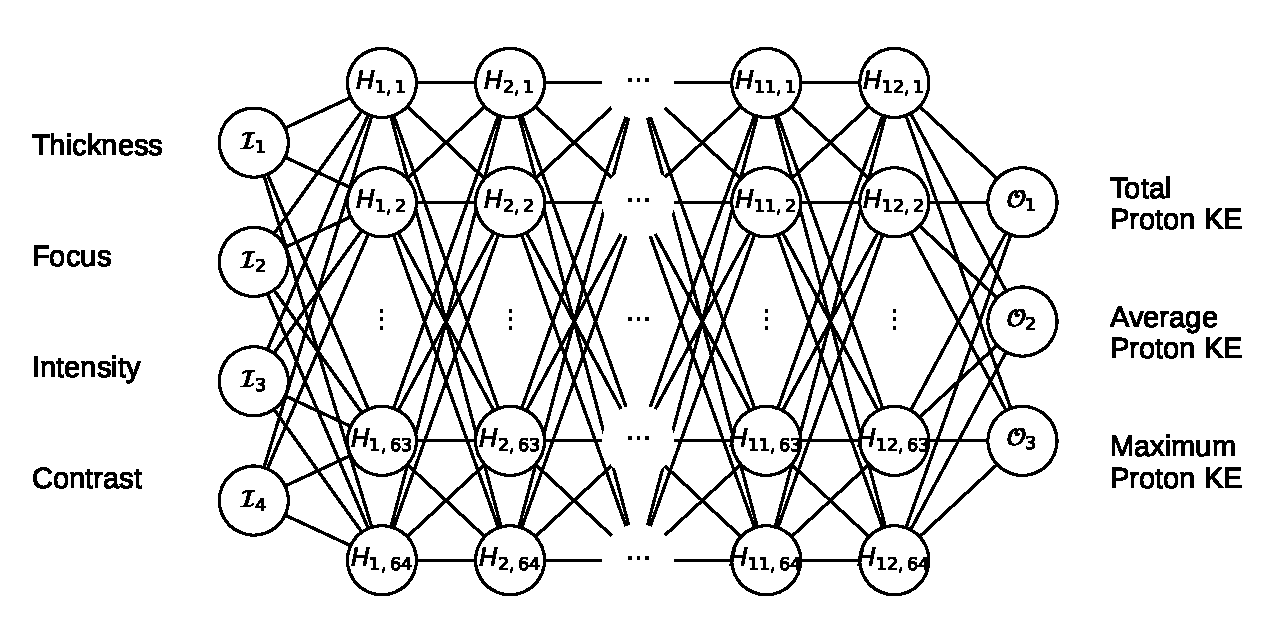
\includegraphics[width=0.95\linewidth]{planning/images/nn_architecture2.eps}
	\caption{The neural network architecture used in \autoref{sec:second_analysis}. This network has 4 inputs, 3 outputs, 12 hidden layers, and 64 neurons per hidden layer.}
	\label{fig:nn_arch}
\end{figure}
